% Figure: AI success rate by proof category
\begin{figure}[t]
\centering
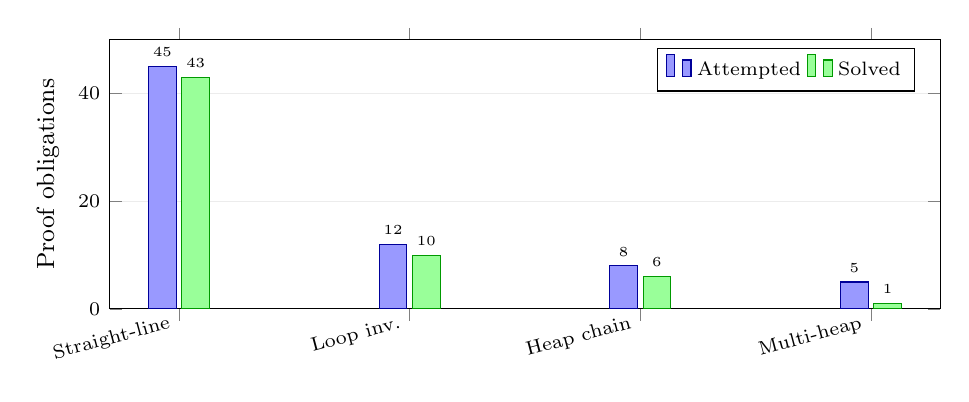
\begin{tikzpicture}
\begin{axis}[
  ybar,
  width=\columnwidth,
  height=5cm,
  bar width=10pt,
  xlabel style={font=\small},
  ylabel={Proof obligations},
  ylabel style={font=\small},
  ymin=0, ymax=50,
  xtick=data,
  xticklabels={Straight-line, Loop inv., Heap chain, Multi-heap},
  xticklabel style={font=\scriptsize, rotate=15, anchor=east},
  tick label style={font=\scriptsize},
  legend style={font=\scriptsize, at={(0.97,0.97)}, anchor=north east,
                legend columns=2},
  grid=major,
  grid style={gray!15},
  ymajorgrids=true,
  xmajorgrids=false,
  nodes near coords,
  nodes near coords style={font=\tiny},
  every node near coord/.append style={anchor=south},
]
\addplot[fill=blue!40, draw=blue!60!black] coordinates {
  (1, 45) (2, 12) (3, 8) (4, 5)
};
\addplot[fill=green!40, draw=green!60!black] coordinates {
  (1, 43) (2, 10) (3, 6) (4, 1)
};
\legend{Attempted, Solved}
\end{axis}
\end{tikzpicture}
\caption{AI success rate by proof category. Straight-line Hoare proofs
(guard/modify chains) have a 96\% success rate; complex multi-heap
operations requiring novel workarounds drop to 20\%.}
\label{fig:ai-success}
\end{figure}
